\documentclass[a4paper]{article}
% Packages
\usepackage{amssymb,amsmath,theorem, tabu}
\usepackage{fullpage}
\usepackage{xcolor,color, colortbl}
\usepackage{enumerate}
\usepackage{tikz}
\usetikzlibrary{decorations.pathmorphing}
\usetikzlibrary{matrix}
\tikzset{snake it/.style={decorate, decoration=snake}}
\usepackage{tkz-euclide}
\usepackage{hhline}
\usepackage[makeroom]{cancel}
% Problem and solution environments
\newtheorem{prob}{\large{\large{Problem}}}
\renewcommand{\theprob}{\arabic{prob}:}
\newcommand\norm[1]{\left\lVert#1\right\rVert}
\newcommand{\notimp}{%
  \mathrel{{\ooalign{\hidewidth$\not\phantom{=}$\hidewidth\cr$\implies$}}}}
\newenvironment{sol}{\noindent{\large{\bf Solution:}}}{\hfill\ensuremath{\square}}

% Some abbreviations
\def\bN{\mathbb N}
\def\bR{\mathbb R}
\def\bQ{\mathbb Q}
\def\bZ{\mathbb Z}
\def\bC{\mathbb C}
\def\bH{\mathbb H}
\def\bP{\mathbb P}
\def\DMO{\DeclareMathOperator}
\DMO{\GL}{GL}
\DMO{\SL}{SL}
\DMO{\gl}{\mathfrak{gl}}
\DMO{\ssl}{\mathfrak{sl}}
\def\rbr#1{\left(#1\right)} %round bracket
\def\imp{\ensuremath{\implies}}
\def\nl{\newline}
\def\bs{\backslash}
\def\pb{\pagebreak}
\def\ns{\varnothing}
\definecolor{redblack}{rgb}{1,0.5,0.5}

\title{MA1126: Set Theory
 Selected Problems}
\author{Anthony Gibbons, Daniel Devine}
\date{February 2019}

\begin{document}

\maketitle

\begin{prob} %Problem 1
\large{ $2016\; Q3$
\begin{enumerate}[(a.)]
\item Define an open set in $\bR$. Define closed set. 
     \nl\begin{sol}
\large{ 
Open set:
\nl A set $A \subset \bR$ is called open if $\forall x\in A,\; \exists \varepsilon>0$ s.t. $N(x,\varepsilon)\subset A$ \\
Where $N(x,\varepsilon)$ is a neighbourhood $\{y\in \bR\;|\; |x-y|<\varepsilon\}$
\nl Closed set:
\nl A set $A\subset \bR$ is closed if $\bR\bs A$ is open, where $\bR\bs A$ is the complement of A in $\bR$
}
\end{sol}
\nl Prove that A is closed $\iff$ it contains all of its accumulation points.
\nl\begin{sol}
\large{\nl$\Rightarrow$
%nl Suppose A is closed, then $X\bs A$ is open
%Then $\forall x\in X\bs A, \exists \varepsilon>0$ s.t. $N(x,\varepsilon)\subset X\bs A$
\nl We need to show that no accumulation points of A are contained in $\bR\bs A$ \\
Accumulation Point: p is an accumulation point of A if \\
$\forall \varepsilon>0 \ \exists \ x\in A\bs\{p\}$ s.t. $|x-p|<\varepsilon$ 

\begin{center}
 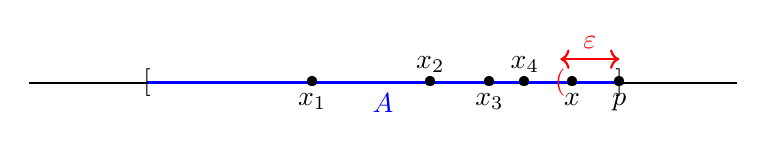
\begin{tikzpicture}[thick,scale=3]
    \coordinate (A1) at (-0.5, 0);
    \coordinate (A2) at (2.5, 0);
    \coordinate (A3) at (0, 0);
    \coordinate (A4) at (2, 0);
    \coordinate (A5) at (1, 0);
    
    \coordinate (E) at (1.875, 0.1);
    \coordinate (E1) at (1.75, 0);
    \coordinate (E2) at (2, 0.1);
    \coordinate (E3) at (1.75, 0.1);
    
    \coordinate (X) at (1.8, 0);
    \coordinate (X1) at (0.7, 0);
    \coordinate (X2) at (1.2, 0);
    \coordinate (X3) at (1.45, 0);
    \coordinate (X4) at (1.6, 0);
    \coordinate (P) at (2, 0);
    
    \draw (A1) -- (A2);
    \draw[blue, very thick] (A3) -- (A4);
    \draw[red, <->] (E2) -- (E3);

%labels
    \node at (A3)  {$[$};
    \node at (A4)  {$]$};
    \node[blue] at (A5) [below] {$A$};
    \node[red] at (E1)  {$($};
    
    \node at (X) {\textbullet};
    \node at (X1) {\textbullet};
    \node at (X2) {\textbullet};
    \node at (X3) {\textbullet};
    \node at (X4) {\textbullet};
    \node at (P) {\textbullet};
    
    \node[red] at (E) [above] {$\varepsilon$};
    \node at (X) [below] {$x$};
    \node at (X1) [below] {$x_1$};
    \node at (X2) [above] {$x_2$};
    \node at (X3) [below] {$x_3$};
    \node at (X4) [above] {$x_4$};
    \node at (P) [below] {$p$};

\end{tikzpicture}
\end{center}
i.e. $\exists$ an infinite sequence $x_1,x_2,x_3,\dots$ of points of A, distinct from p, that converge to p, with $\lim\limits_{j\to\infty}x_j=p$ 
but all $x_j\in A$, hence $p\in A$ also
\nl Hence A contains all of its accumulation points
\nl A is closed $\imp$ it contains all of its accumulation points.
\nl$\Leftarrow$
Now assume A contains all of its accumulation points, then choose $p \in \bR\bs A,$ so p is not an accumulation point of A.
\nl So by definition of accumulation points, $\exists \delta>0$ s.t. $\{x \in A\:|\: 0 < |x-p| < \delta\}=\ns$
\nl Hence there exists an open ball about p in $\bR\bs A$, so $\bR\bs A$ is open,$\imp A$ is closed
\nl So A is closed $\iff$ it contains all of its accumulation points, as required.}
\end{sol}
\item Define Cauchy sequence.
 \nl\begin{sol}
\large{ 
A Cauchy sequence $a_1,a_2,a_3,\dots$\quad (infinite sequence) such that $\forall \varepsilon>0\exists N\in \bN s.t. |a_n-a_m|<\varepsilon \forall n,m\geq N$

}
\end{sol}
\item Prove that every Cauchy Sequence converges in $\bR$ is equivalent to the least upper bound axiom
 \nl\begin{sol}
\large{ 
Want $C.S.\imp L.U.B\; and\; L.U.B\imp C.S.$
Assume Cauchy convergence.
\nl Let A be a nonempty subset of $\bR$ and suppose A has an upper bound $b_1$
\nl Since A is nonempty, $\exists a_1 \in A$ and not an upper bound.
\nl Define sequences $a_1,a_2,a_3,\dots \qquad b_1,b_2,b_3,\dots$ as follows:
\nl Check if $\frac{a_n+b_n}{2}$ is an upper bound of A.
\nl If so, $a_{n+1}=a_n,\quad b_{n+1}=\frac{a_n+b_n}{2}$
\nl Otherwise, $\exists s\in A s.t. \ s>\frac{a_n+b_n}{2}$
\nl Let $a_{n+1}=s, b_{n+1}=b_n$
\begin{center}
 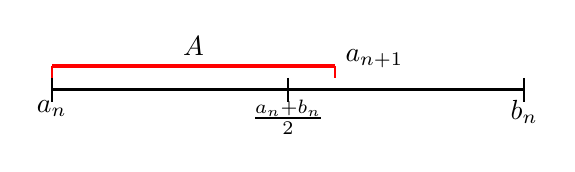
\begin{tikzpicture}[thick,scale=3]
    \coordinate (A1) at (0, 0);
    \coordinate (A2) at (2, 0);
    \coordinate (A3) at (1, 0);
    \coordinate (A4) at (1.2, 0.1);
    \coordinate (A5) at (0.6, 0.1);
    \coordinate (B1) at (0, 0.1);
    
    \coordinate (C1) at (0, 0.1);
    \coordinate (C2) at (0, 0.05);
    \coordinate (C3) at (0, -0.05);
    \coordinate (C4) at (1, 0.05);
    \coordinate (C5) at (1, -0.05);
    \coordinate (C6) at (2, 0.05);
    \coordinate (C7) at (2, -0.05);
    \coordinate (C8) at (1.2, 0.05);



    \draw[very thick] (A1) -- (A2);
    \draw[very thick] (A2) -- (A3);
    \draw[red, very thick] (A4) -- (B1);
    \draw[red] (C1) -- (C2);
    \draw[red] (C8) -- (A4);
    \draw (C2) -- (C3);
    \draw (C4) -- (C5);
    \draw (C6) -- (C7);


%labels
    \node at (A1) [below] {$a_n$};
    \node at (A2) [below] {$b_n$};
    \node at (A3) [below] {$\frac{a_n+b_n}{2}$};
    \node at (A5) [above] {$A$};
    \node at (C8) [above right] {$a_{n+1}$};

\end{tikzpicture}
\end{center}
Then $a_1\leq a_2\leq \dots \leq b_2\leq b_1$ and $|b_n-a_n|\to 0$ as $n\to \infty$
\nl\imp Both sequences are Cauchy $\therefore$ they converge towards some limit L\\
\imp L is the least upper bound for s \checkmark\\
Note: Every Cauchy sequence is bounded.\\
\underline{Proof:} \\
Take $\varepsilon=1$, then \\
$\exists \ N\in \bN s.t. \ m,n\geq N \imp |x_m-x_n|<1 \imp |x_m|-|x_n|<1 \imp |x_m|<1+|x_n|$\\
In general, $|x_n|\leq max\{|x_1|,\dots,|x_n|,1+|x_n|\}$\\
Note also that every sequence has a monotone (strictly increasing) subsequence.\\ \\
Now Assume Least upper bound axiom is true.\\
Suppose we have a monotone bounded sequence (increasing)\\
Since it is bounded, by the L.U.B axiom, then it has a supremum.\\ $s=\sup\limits_{n\in \bN}\{x_n\}$\\
Claim S is the limit of the sequence.\\
Let $\varepsilon>0$, then $\exists N\in \bN$ s.t. $s-\frac{\varepsilon}2<x_N\leq x_{N+1}\leq\dots\leq S$
\nl\imp $\forall n\geq N$ we have $|x_n-s|<\frac{\varepsilon}{2}$
\nl Now take any $x_m$ in the original sequence with $m>N$ \\
$|x_m-x_n|\leq |x_m-s|+|x_n-s|<\frac{\varepsilon}{2}+\frac{\varepsilon}{2}=\varepsilon$\\ 
So the sequence is Cauchy \checkmark
}
\end{sol}
\end{enumerate}
}
   
\end{prob}
\pagebreak

\begin{prob} %Problem 2
\large{$2017\; Q4$
\begin{enumerate}[(a.)]
\item Show that $f:\bR\to\bR$ is continuous $\iff$ the preimage of any open set  $U, f^{-1}(U)$ is open
\nl \begin{sol}
\large{ \\$\Rightarrow$
\nl Assume f is continuous on $\bR$, then 
\nl $\forall x_0\in \bR, \forall\varepsilon>0, \exists \delta>0 s.t. |x-x_0|<\delta \imp |f(x)-f(x_0)|<\varepsilon$
\nl In other words, $\forall x_0 \in \bR, \forall N(f(x_0),\varepsilon) \exists N(x_0,\delta)s.t. f(N(x_0,\delta))\subset N(f(x_0),\varepsilon)$
\nl Let U be open in $\bR$
\nl Let $x_0\in f^{-1}(U)$
\nl Then $f(x_0)\in U$
\nl\imp $\exists \varepsilon>0 s.t. N(f(x_0),\varepsilon)\subset U
\nl\imp \exists N(x_0,\delta) s.t. f(N(x_0,\delta))\subset N(f(x_0),\varepsilon)\subset U
\nl\imp N(x_0,\delta)\subset f^{-1}(U)$
\nl $x_0$ is an interior point of $f^{-1}(U)\imp f^{-1}(U)$ is open. 
\nl $\Leftarrow 
\nl f^{-1}(U)$ for any U open.
\nl Given $N(f(x_0),\varepsilon),$ this is open.
\imp $f^{-1}(N(f(x_0),\varepsilon))$ is open.
\nl and $x_0 \in f^{-1}(N(f(x_0),\varepsilon))$ so $x_0$ is an interior point
\nl\imp $\exists \delta>0 s.t. N(x_0,\delta)\subset f^{-1}(N(f(x_0),\varepsilon))
\nl\imp f(N(x_0,\delta)\subset N(f(x_0),\varepsilon)$ \imp f is continuous.
}
\end{sol}
\item Prove that the continuous image of a compact subset of R is compact.
\nl \begin{sol}
\large{ Suppose $A\subset \bR$ is compact, and f is continuous
\nl Suppose $f(A)\subset\bigcup\limits_\alpha U_\alpha, U_\alpha open$
\nl Then $A\subset f^{-1}(\bigcup\limits_\alpha U_\alpha)=\bigcup\limits_\alpha f^{-1}(U_\alpha)$
\nl By part (a.), each of the $f^{-1}(U_\alpha)$ is open.
\nl And A is compact $\imp \exists$ a finite subcover of A
\nl .e. $A\subset f^{-1}(U_{\alpha_1})\cup f^{-1}( U_{\alpha_2})\cup\dots\cup f^{-1}( U_{\alpha_n})$
\nl \imp $f(A)\subset U_{\alpha_1}\cup U_{\alpha_1}\cup \dots U_{\alpha_n} \imp f(A)$ is compact.
}
\end{sol}
\item Use part (b.) to prove the Extreme Value Theorem
\nl\begin{sol}
\nl \large{ Suppose f is continuous on $[a,b], \nl [a,b]$ is compact by Heine-Borel.
\nl Then f([a,b]) is compact by part (b.)\imp it is closed and bounded.
\nl\quad bounded\imp LUB and GLB exist
\nl\quad closed\imp LUB and GLB belong to $f([a,b])$
\nl So $\exists x_0,x\in[a,b]$ s.t. $f(x_0)=\max\limits_{x\in[a,b]}f(x)\qquad f(x_1)=\min\limits_{x\in[a,b]}f(x)$
\nl This is the Extreme Value Theorem.
}
\end{sol}
\end{enumerate}
}

\end{prob}
\pagebreak
\begin{prob} %Problem 3
\large{$2017\; Q3$
\begin{enumerate}[(a.)]
\item Prove or disprove
\begin{enumerate}[1.]
    \item $U_n open \ \forall n\geq 1 \imp \bigcap\limits_{n\geq 1}U_n$ open.
\nl\begin{sol}
\large{ 
$U_n open \ \notimp \bigcap\limits_{n\geq 1}U_n$ open.\\
e.g. let $U_n=(-\frac1n,\frac1n)$\\
$\bigcap\limits_{n\geq 1}U_n=\{0\}$ which is not open.
}
\end{sol}    
    \item $U_n \ open \ \forall n\geq 1 \imp \bigcup\limits_{n\geq 1}U_n$ open.
\nl\begin{sol}
\large{ Let $x\in \bigcup\limits_{n\geq 1}U_n \imp x \in U_{n_i}$ for some $n_i$\\
\imp $\exists \varepsilon>0$ s.t. $N(x,\varepsilon)\subset U_{n_i}\\
\imp N(x,\varepsilon)\subset \bigcup\limits_{n\geq 1}U_n\\
\imp \bigcup\limits_{n\geq 1}U_n$ is open.

}
\end{sol}    
    \item $U_n closed \ \forall n\geq 1 \imp \bigcap\limits_{n\geq 1}U_n$ closed.
\nl\begin{sol}
\large{ $U_n$ closed $\imp (U_n)^C open\\
\imp \bigcup\limits_{n\geq 1}(U_n)^C$ is open, from above.\\
\imp $(\bigcup\limits_{n\geq 1}(U_n)^C)^C\\
\imp \bigcap\limits_{n\geq1}(U_n^C)^C=\bigcap\limits_{n\geq1}(U_n)$ closed.
}
\end{sol}    
    \item $U_n closed \ \forall n\geq 1 \imp \bigcup\limits_{n\geq 1}U_n$ closed.
\nl\begin{sol}
\large{ $U_n closed \ \notimp \bigcup\limits_{n\geq 1}U_n$ closed.\\
e.g. $O_n=\{\frac1n\}$
0 is an accumulation point not included in $\bigcup\limits_{n\geq 1}U_n$ \\
\imp not closed (since a set is closed $\iff$ it contains all its accumulation points.

}
\end{sol}   
\end{enumerate}

\item Prove a subset of R is compact $\iff$ it is closed and bounded
\nl\begin{sol}
\large{\\ $\Rightarrow$
\nl Suppose $A\subset \bR$ Suppose it is not bounded\\
Let $U_n=(-n,n) \qquad Then\; A\subset \bigcup U_n=\bR$\\
But a finite subcover cannot be found \imp A is not compact\\
So not bounded \imp not compact\\
\nl Taking the contrapositive
compact \imp bounded.
\nl Suppose $A\subset \bR$ and not closed
$\exists x$ an accumulation point of A not in A\\
\nl Let $U_n=(-\infty,x-\frac{1}{n})\cup(x+\frac{1}{n},+\infty)$ be a cover of A
\begin{center}
 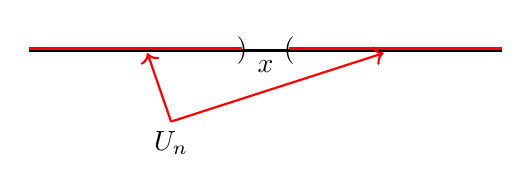
\begin{tikzpicture}[thick,scale=3]
    \coordinate (A1) at (0, 0);
    \coordinate (A2) at (2, 0);
    \coordinate (A3) at (1, 0);
    \coordinate (A4) at (0.9, 0);
    \coordinate (A5) at (1.1, 0);
    
    \coordinate (B1) at (0.6, -0.3);
    \coordinate (B2) at (0.5, -0.01);
    \coordinate (B3) at (1.5, -0.01);
    
    \coordinate (C1) at (0, 0.01);
    \coordinate (C2) at (0.9, 0.01);
    \coordinate (C3) at (1.1, 0.01);
    \coordinate (C4) at (2, 0.01);



    \draw[very thick] (A1) -- (A2);
    \draw[red, very thick] (C3) -- (C4);
    \draw[red, very thick] (C1) -- (C2);
    \draw[red, ->] (B1) -- (B2);
    \draw[red, ->] (B1) -- (B3);

%labels
    \node at (A3) [below] {$x$};
    \node at (A4)  {$)$};
    \node at (A5)  {$($};
    \node at (B1)  [below]{$U_n$};

\end{tikzpicture}
\end{center}
But a finite subcover cannot be found \imp A not compact\\
So not closed \imp not compact
\nl Taking the contrapositive
compact \imp closed.
\nl $\Leftarrow$
\nl Now suppose A is closed and bounded.
\nl \underline{Case 1:} $A=[a,b]$
\nl Suppose $A\subset \bigcup\limits_\alpha U_\alpha$ and a finite number of $U_\alpha$ don't cover $A=I_1$
\begin{center}
 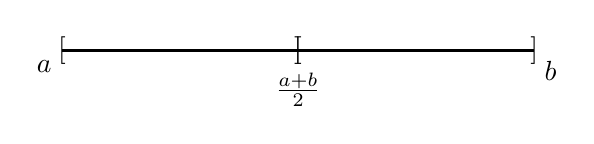
\begin{tikzpicture}[thick,scale=3]
    \coordinate (A1) at (0, 0);
    \coordinate (A2) at (2, 0);
    \coordinate (A3) at (1, 0);
    \coordinate (A4) at (1, -0.05);
    
    \draw[very thick] (A1) -- (A2);

%labels
    \node at (A4) [below] {$\frac{a+b}2$};
    \node at (A3)  {$]$};
    \node at (A3)  {$[$};
    \node at (A1)  {$[$};
    \node at (A2)  {$]$};
    \node at (A2)  [below right]{$b$};
    \node at (A1)  [below left]{$a$};

\end{tikzpicture}
\end{center}
Consider $[a,\frac{a+b}2]$ and $[\frac{a+b}2,b]$
\nl One of these subintervals which we will call $I_2$, also does not have a finite subcover.
\nl Divide $I_2$ in half, one of these will not have a finite subcover $\dots$ etc.
\nl We have $I_1\supset I_2 \supset I_3 \supset \dots \supset I_n \supset \dots$ infinite series of nested subintervals. 
\nl with each $I_n$ closed and bounded interval that does not have a finite subcover of $U_\alpha$
\nl By the Nested Intervals Theorem, $\bigcap I_n\neq\ns$
\nl Let $x\in \bigcap I_n$, so $x\in U_{\alpha_i}$ for some $\alpha_i$
\nl $U_{\alpha_i}$ open, then $\exists \varepsilon>0 \; s.t.\; N(x,\varepsilon)\subset U_{\alpha_i}$
\nl $But |I_n|\to 0$ and if $|I_n|<\varepsilon,$ then $x\in I_n \imp I_n\subset N(x,\varepsilon)$
\nl\imp $I_n$ has a finite subcover $\Rightarrow\Leftarrow$ Contradiction
\nl Then A is closed
\nl \underline{Case 2:}
\nl A is closed and bounded but not necessarily an interval.
\nl If $A\subset \bigcup U_\alpha \qquad \exists [a,b]\;s.t.\; A\subset[a,b]$
\nl and if we consider all $U_\alpha$ and $A^C$, we have an open cover of $[a,b]$.
\nl\imp $\exists$ a finite subcover $U_{\alpha_1}\cup\dots\cup U_{\alpha_n}$ ($\cup A^C$ possibly)
\nl But $A\cup A^C = \ns \therefore U_{\alpha_1}\cup\dots\cup U_{\alpha_n}\supset A$ covers A
}
\end{sol}
\end{enumerate}
}

\end{prob}
\pagebreak
\begin{prob} %Problem 4
\large{Page $16\; Q48$
\nl we define $\oplus$ to denote exclusive or, so $p\oplus q \equiv (p\lor Q)\land \lnot(p\land q)$
\nl Hence the truth table for exclusive or is as follows:

    $\begin{tabu}{|cc||c|}
    \hline
      p & q & p\oplus q \\ \hhline{|==||=|}
      T & T & F \\ 
      T & F & T \\ 
      F & T & T \\ 
      F & F & F \\ \hline
         
    \end{tabu}$

\begin{enumerate}[a.]
    \item find simpler statement forms that are logically equivalent to $p \oplus p$ and $(p \oplus p) \oplus p$
    \nl\begin{sol}
\nl\large{ $\begin{tabu}{|cc||c|}
    \hline
      p & (p\oplus p) & (p\oplus p)\oplus p \\ \hhline{|==||=|}
      T & F & T \\ 
      F & F & F \\ \hline
         
    \end{tabu}$\\
   
  So $(p\oplus p) \equiv$ contradiction,\qquad $(p\oplus p)\oplus p \equiv p$
}
\end{sol}
    \item Is $(p\oplus q)\oplus r\equiv (p\oplus q)\oplus r$? Justify your answer.\\
    \begin{sol}
\nl\large{ $\begin{tabu}{|c|c|c|c|c|c|c|}
    \hline
      p & q & r & (p\oplus q) & (p\oplus q)\oplus r & (q\oplus r) & p\oplus (q\oplus r) \\ \hhline{|=|=|=|=|=|=|=|}
      T & T & T & F & T & F & T  \\ 
      T & T & F & F & F & T & F  \\ 
      T & F & T & T & F & T & F  \\ 
      T & F & F & T & T & F & T  \\ 
      F & T & T & T & F & F & F  \\ 
      F & T & F & T & T & T & T  \\ 
      F & F & T & F & T & T & T  \\ 
      F & F & F & F & F & F & F  \\  \hline
    \end{tabu}$\\
   
  So $(p\oplus q)\oplus r\equiv (p\oplus q)\oplus r$
}
\end{sol}
    \item Is $(p\oplus q)\land r\equiv (p\land q)\oplus (q\land r)$? Justify your answer.
    \nl\begin{sol}\nl
\nl\large{ $\begin{tabu}{|c|c|c|c|c|c|c|c|}
    \hline
      p & q & r & (p\oplus q) & (p\oplus q)\land r & (p \land r) & (q\land r) & {(p \land r) \oplus (q\land r)}  \\ \hhline{|=|=|=|=|=|=|=|=|}
      T & T & T & F & F & T & T & F \\ 
      T & T & F & F & F & F & F & F \\ 
      T & F & T & T & T & T & F & T \\ 
      T & F & F & T & F & F & F & F \\ 
      F & T & T & T & T & F & T & T \\ 
      F & T & F & T & F & F & F & F \\ 
      F & F & T & F & F & F & F & F \\ 
      F & F & F & F & F & F & F & F \\  \hline
    \end{tabu}$\\
   
  So $(p\oplus q)\land r\equiv (p\land q)\oplus (q\land r)$
  }
  \end{sol}
\end{enumerate}
}
\end{prob}
\pagebreak
\begin{prob} %Problem 5
\large{ $2018\; Q2$
\begin{enumerate}[(a.)]
\item Define what it means for 2 sets to have the same cardinal number. 
\nl\begin{sol}
\large{ 2 sets X and Y have the same cardinality if $\exists$ a bijective map $f:X\to Y$ i.e. a 1-1 correspondence.
}
\end{sol}\\
Define Cardinal Number.
\nl\begin{sol}
\large{ The cardinal number of a set X, \#X is the number of elements in the set X \\
e.g. $\#\{1,2,4,6,9\}=5$
}
\end{sol}\\
Prove that $\bQ$ is countable but $\bR$ is not.
     \nl\begin{sol}
\large{ 
\begin{enumerate}[1.]
    \item Define $\bQ_{+}$=\\
\begin{tikzpicture}
\matrix(m)[matrix of math nodes,column sep=1cm,row sep=1cm]{
    s_{1,1} & s_{1,2} & s_{1,3} & s_{1,4} & \cdots \\
    s_{2,1} & s_{2,2} & s_{2,3} & s_{2,4} & \cdots \\
    s_{3,1} & s_{3,2} & s_{3,3} & s_{3,4} & \cdots \\
    s_{4,1} & s_{4,2} & s_{4,3} & s_{4,4} & \cdots \\
    \vdots &  \vdots &  \vdots &  \vdots & \ddots \\
};

\draw[red, ->]
         (m-1-1)edge(m-1-2)
         (m-1-2)edge(m-2-1)
         (m-2-1)edge(m-3-1)
         (m-3-1)edge(m-2-2)
         (m-2-2)edge(m-1-3)
         (m-1-3)edge(m-1-4)
         (m-1-4)edge(m-2-3)
         (m-2-3)edge(m-3-2)
         (m-3-2)edge(m-4-1)
         (m-4-1)edge(m-5-1);
\end{tikzpicture}
\\ Where $s_{ij}=\frac{i}{j}, j\neq 0$, i.e.\\
\begin{tikzpicture}
\matrix(m)[matrix of math nodes,column sep=1cm,row sep=1cm]{
    \frac11 & \frac12 & \frac13 & \frac14 & \cdots \\
    \frac21 & \frac22 & \frac23 & \frac24 & \cdots \\
    \frac31 & \frac32 & \frac33 & \frac34 & \cdots \\
    \frac41 & \frac42 & \frac43 & \frac44 & \cdots \\
    \vdots &  \vdots &  \vdots &  \vdots & \ddots \\
};

\draw[red, ->]
         (m-1-1)edge(m-1-2)
         (m-1-2)edge(m-2-1)
         (m-2-1)edge(m-3-1)
         (m-3-1)edge(m-2-2)
         (m-2-2)edge(m-1-3)
         (m-1-3)edge(m-1-4)
         (m-1-4)edge(m-2-3)
         (m-2-3)edge(m-3-2)
         (m-3-2)edge(m-4-1)
         (m-4-1)edge(m-5-1);
\end{tikzpicture}
\\We define the list in the diagonalising order as defined in the diagram, where we skip the rational numbers already in the list, e.g.$\frac22=\frac11\quad \frac84=\frac21$\\
Hence $\bQ_{+}$ is countable. Similarly, $\bQ_{-}$ is countable.
Hence $\bQ=\bQ_{+}\cup\{0\}\cup\bQ_{-}$ is countable.

\item We show below in part (c.) that $\prod_{i=1}^\infty \{0,1\} \sim \bP(\bN)$ and that $\#\bP(\bN)>\#\bN$\\
Claim the interval $(0,1)$ is not countable. If not, then $\bR$ is not countable.\\ 
Assume $\bR$ is countable. We consider the countable list of decimal expansions \\
$\begin{tabu}{ccccccc}
  a^1= &  \cdot & a_{11} & a_{12} & a_{13} & a_{14} & \cdots \\
  a^2= &  \cdot & a_{21} & a_{22} & a_{23} & a_{24} & \cdots \\
  a^3= &  \cdot & a_{31} & a_{32} & a_{33} & a_{34} & \cdots \\
  a^4= &  \cdot & a_{41} & a_{42} & a_{43} & a_{44} & \cdots \\
  \vdots& \cdot       & \vdots & \vdots & \vdots & \vdots & \ddots
\end{tabu}$\\ Where $0\leq a_{ij} \leq 9 \ \forall \ i,j\geq 1$
Define a decimal expansion 
$$b=\cdot (a_{11}+1)\;(a_{22}+1)\;(a_{33}+1)\;(a_{44}+1)\;\cdots\;(a_{nn}+1)\;\cdots$$ But $9\to 1$ as we don't want a string of zeroes\\
This is a real number by completeness of the real line,
This is not equal to any of the decimal expansions above since it is different to each of the $a^i$ in the $i^{th}$ place. Hence $(0,1)$ is not countable $\therefore \bR$ is not countable.
\end{enumerate}
}
\end{sol}
\nl 
\item State the Schroeder-Bernstein Theorem and Cantor's Theorem. 
\nl\begin{sol}
\large{ \underline{Schroeder-Bernstein Theorem} 
\\ If $\exists f: X\to Y$ one to one
\\ If $\exists g: Y\to X$ one to one
\\ Then $\exists h: X\to Y$ one to one and onto.
\\ i.e. $\#X\leq \#Y \ and \ \#Y\leq \#X \imp \#X=\#Y$
\\ \\ \underline{Cantor's Theorem}
\\ For any set A, $\#A<\#\bP(A) \ i.e. \ n<2^n$
\\ i.e. $\not\exists f:A\to \bP(A)$ one to one and onto.
}
\end{sol}
\nl Prove Cantor's Theorem.
 \nl\begin{sol}
 
\large{ Suppose There exists $f:A\to \bP(A)$ one to one and onto.
\\ Let $B=\{x\in A \:|\: x \notin f(x)\} \therefore B\subset A$
\\ $B\subset A \imp B\in \bP(A)$
\\ f surjective $\imp \exists$ y s.t. $f(y)=B
\\ Suppose\; y\in B, y\in f(y) \imp y\notin B
\Rightarrow\Leftarrow \;contradiction.
\\ Suppose\; y\notin B, y\notin f(y) \imp y\in B
\Rightarrow\Leftarrow \;contradiction.$
\\ $\therefore$ f does not exist.
}
\end{sol}
\item Prove $\prod_{i=1}^\infty \{0,1\} \sim \bP(\bN)$
 \nl\begin{sol}
\large{ This means there exists a bijective map $f: \prod_{i=1}^\infty \{0,1\} \to \bP(\bN)$\\
$\prod_{i=1}^\infty \{0,1\}$ is a sequence of 0's and 1's. e.g.$\{1,0,1,0,0,\dots\}$\\
$A\subset \bN \to f(A)\in \prod_{i=1}^\infty \{0,1\}$\\
e.g. $\{1,3,7\}$=
$\begin{tabu}{cccccccccccc}
  \{ & 1, & 0, & 1, & 0, & 0, & 0, & 1, & 0, & 0,  & \dots &\} \\
 \rowfont{\color{red}}
     & 1  & \not2  & 3  & \not4  & \not5  & \not6  & 7  & \not8 & \not9, & \dots  
\end{tabu}$\\
So the sequence $\{f(A)\}_i=\begin{cases}
1, & if \ i\in A\\
0, & if \ i\notin A
\end{cases}$\\
Is f bijective?\\
\underline{Injective:} Does $f(A_1)=f(A_2)\imp A_1=A_2$?\\
Let $j\in A_1 \imp f(A_1)_j=1=f(A_2)_j$
\imp $j\in A_2$\\
So $A_1\subset A_2$\\
By symmetry, $A_2\subset A_1$ also\\
\imp $A_1=A_2 \therefore$ injective.\\
\underline{Surjective:} given $b=\{b_1,b_2,b_2,\dots\}\in \prod_{i=1}^\infty \{0,1\}$\\
Does there exist $A\subset \bN$ s.t. $f(A)=b$?\\
We know $j\in A \iff b_j=1\\
f(A)_j-1\iff j\in A \iff b_j=1 \forall j \\
\therefore f(A)_j=b_j \forall j \\
\imp f(A)=b \therefore$ surjective\\
Hence f is bijective, and $\prod_{i=1}^\infty \{0,1\} \sim \bP(\bN)$
}
\end{sol}
\end{enumerate}
}
\textbf{Extra:} Prove the Schroeder-Bernstein Theorem 
\nl\begin{sol}
\large{ 

In the below diagram we use the fact that $f(X\bs Y)=f(X)\bs f(Y)$

\begin{center}
 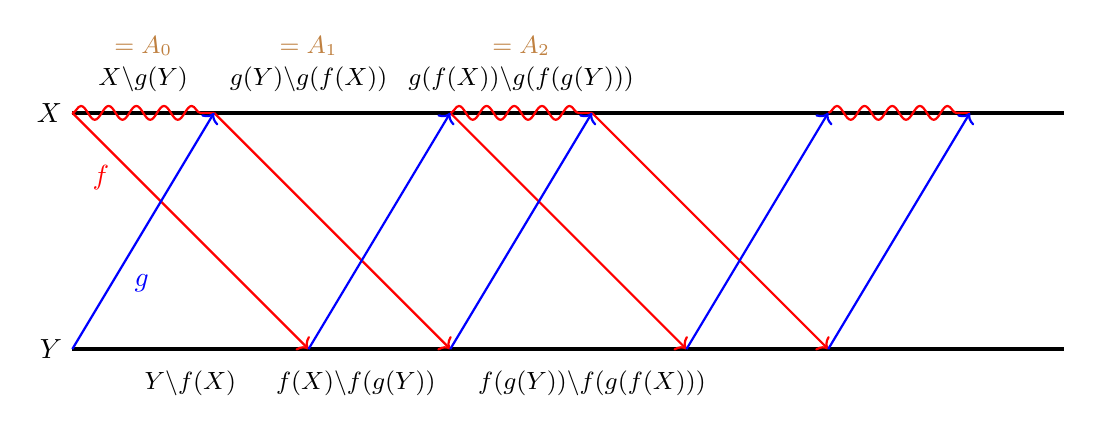
\begin{tikzpicture}[thick,scale=3]
 
    \coordinate (X) at (-1, 0);
    \coordinate (Y) at (-1, -1);
 
    \coordinate (A0) at (0, 0);
    \coordinate (A1) at (0.6, 0);
    \coordinate (A2) at (1.6, 0);
    \coordinate (A3) at (2.2, 0);
    \coordinate (A4) at (3.2, 0);
    \coordinate (A5) at (3.8, 0);
    \coordinate (A6) at (4.2, 0);

    \coordinate (B0) at (0, -1);
    \coordinate (B1) at (1, -1);
    \coordinate (B2) at (1.6, -1);
    \coordinate (B3) at (2.6, -1);
    \coordinate (B4) at (3.2, -1);
    \coordinate (B5) at (4.2, -1);
    
    \coordinate (C0) at (0.3, 0.05);
    \coordinate (C1) at (1, 0.05);
    \coordinate (C2) at (1.9, 0.05);
    \coordinate (C3) at (3.1, 0.05);
    
    \coordinate (D0) at (0.5, -1.05);
    \coordinate (D1) at (1.2, -1.05);
    \coordinate (D2) at (2.2, -1.05);
    \coordinate (D3) at (2.9, -1.05);
    
    \coordinate (E0) at (0.3, 0.2);
    \coordinate (E1) at (1, 0.2);
    \coordinate (E2) at (1.9, 0.2);


    %\draw[very thick] (A1) -- (A2);
    %\draw[very thick] (A2) -- (A3);
    %\draw[red, very thick] (A4) -- (B1);
    %\draw[red] (C1) -- (C2);
    %\draw[red] (C8) -- (A4);
    %\draw (C2) -- (C3);
    %\draw (C4) -- (C5);
    %\draw (C6) -- (C7);
    
    \coordinate (F) at (0.2, -0.18);
    \coordinate (G) at (0.22, -0.8);
    
    \draw[very thick] (A0) -- (A6);
    \draw[very thick] (B0) -- (B5);
    
    \path [draw=red,snake it]
    (A0) -- (A1);
    \path [draw=red,snake it]
    (A2) -- (A3);
    \path [draw=red,snake it]
    (A4) -- (A5);
 % \draw[draw=blue, snake it] (2,0) arc (0:180:2cm);
    
    
    \draw[red, ->] (A0) -- (B1);
    \draw[red, ->] (A1) -- (B2);
    \draw[red, ->] (A2) -- (B3);
    \draw[red, ->] (A3) -- (B4);
    %\draw[red, ->] (A4) -- (B5);
    %\draw[red, ->] (A5) -- (B6);
    
    \draw[blue, ->] (B0) -- (A1);
    \draw[blue, ->] (B1) -- (A2);
    \draw[blue, ->] (B2) -- (A3);
    \draw[blue, ->] (B3) -- (A4);
    \draw[blue, ->] (B4) -- (A5);
    %\draw[blue, ->] (B5) -- (A6);

%labels
    \node at (A0) [left] {$X$};
    \node at (B0) [left] {$Y$};
    \node [red] at (F) [below left] {$f$};
    \node [blue] at (G) [above right] {$g$};
    
    \small{
    \node at (C0) [above] {$X\bs g(Y)$};
    \node at (C1) [above] {$g(Y)\bs g(f(X))$};
    \node at (C2) [above] {$g(f(X))\bs g(f(g(Y)))$};
    %\node at (C3) [above] {$g(f(g(Y)))\bs g(f(g(f(X))))$};
    
    \node at (D0) [below] {$Y\bs f(X)$};
    \node at (D1) [below] {$f(X)\bs f(g(Y))$};
    \node at (D2) [below] {$f(g(Y))\bs f(g(f(X)))$};
    
    \node [brown] at (E0) [above] {$=A_0$};
    \node [brown] at (E1) [above] {$=A_1$};
    \node [brown] at (E2) [above] {$=A_2$};
    %\node at (D3) [below] {$f(g(f(X)))\bs f(g(f(g(Y))))$};
}
\end{tikzpicture}
\end{center}
$X=X\bs g(Y)\;\cup\; g(Y)\bs g(f(X))\;\cup\; g(f(X))\bs g(f(g(Y)))\;\cup\; \dots \\
Y=Y\bs f(X)\;\cup\; f(X)\bs f(g(Y))\; \cup\; f(g(Y))\bs f(g(f(X)))\;\cup\;\dots$\\
$A_{n+1}=g(f(A_n))\; and\; A_\infty =\bigcup\limits_{n=0}^\infty A_n$\\
Define $$
h(x)=
\begin{cases}
f(x), & if \ x \in A_\infty\\
g^{-1}(x), & \ otherwise
\end{cases}
$$
We can easily show h is onto since all of Y is used\\
But is h injective?
%$f(X)=f[X\bs g(Y)\;\cup\; g(Y)\bs g(f(X))\;\cup\; g(f(x))\bs g(f(g(Y)))\;\cup\; \dots]
%\nl=f(X\bs g(Y))\;\cup\; f(g(Y)\bs g(f(X)))\;\cup\; f(g(f(x))\bs g(f(g(Y))))\;\cup\; \dots
%\nl=f(X)\bs f(g(Y)))\;\cup\; f(g(Y))\bs f(g(f(X))))\;\cup\; f(g(f(x)))\bs f(g(f(g(Y)))))\;\cup\; \dots$
\nl We are also using the result that if h is injective on $A_1,A_2$, then h is injective on $A_1 \cup A_2$ if $f(A_1)\cap f(A_2)=\ns$.\\
Hence $A_\infty$ is the union of disjoint $A_n$, and h is injective on all the $A_n$ since f is. so h is injective on the $A_\infty$.\\
Similarly h is injective $\forall x \notin A_\infty$ by injectivity of g.\\
So h is injective $\forall x\in X$
\nl \imp h is bijective, as required
}
\end{sol}
\end{prob}
\end{document}
